\documentclass[aspectratio=169, t]{beamer}

\usepackage{amsmath}
\usepackage{amssymb}
\usepackage{graphicx}
\usepackage{tikz}
\usetikzlibrary{positioning}
\usepackage{xcolor}

% Theme
\usetheme{Madrid}
\usecolortheme{default}

% Layout
\setbeamersize{text margin left=1.0cm, text margin right=1.0cm}
\setbeamertemplate{navigation symbols}{}
\setlength{\parskip}{0.2em}
\setlength{\itemsep}{0.25em}

% Custom colors
\definecolor{darkblue}{RGB}{25, 45, 85}
\definecolor{lightblue}{RGB}{173, 216, 230}
\definecolor{darkgreen}{RGB}{34, 102, 68}
\definecolor{lightgreen}{RGB}{144, 238, 144}
\definecolor{orange}{RGB}{255, 165, 0}
\definecolor{coral}{RGB}{255, 127, 80}
\definecolor{gold}{RGB}{218, 165, 32}

\setbeamercolor{palette primary}{bg=darkblue, fg=white}
\setbeamercolor{palette secondary}{bg=lightblue, fg=darkblue}
\setbeamercolor{palette tertiary}{bg=darkgreen, fg=white}
\setbeamercolor{structure}{fg=darkblue}
\setbeamercolor{titlelike}{bg=darkblue, fg=white}

% Title page info
\title{Towards a Universal Brain Model}
\subtitle{Multi-Modal Progression Modeling}
\author{HAIM 4}
\date{\today}

\begin{document}

\begin{frame}
  \titlepage
\end{frame}

% ====================
% SLIDE 1: DATA
% ====================
\begin{frame}{Data}

  \textbf{Modalities:} MRI, CT, Angiogram

  \medskip

  \renewcommand{\arraystretch}{1.25}
  \begin{tabular}{@{}lll@{}}
    \textbf{Dataset} & \textbf{Scan type} & \textbf{Target} \\
    \hline
    PhysioNet (82) & 2D CT & ICH segmentation \\
    BHSD (192 + 2200 unlabeled) & 2D CT & ICH segmentation \\
    RSNA (25k) & 2D CT & ICH classification \\
    CQ500 (491) & 2D CT & ICH classification \\
    fastMRI (7k) & MRI & -- \\
    ISLES (250) & 2D CT + Tabular & Stroke Progression \\
    APIS (100) & 2D CT + MRI Pairs & Stroke \\
    Hartford datasets (25k+) & 3D CT / MRI / Angio & Temporal pairs \\
  \end{tabular}

\end{frame}

% ====================
% SLIDE 2: OBJECTIVE
% ====================
\begin{frame}{Objective}

  \textbf{\large Learn progression of brain pathology across time and modalities}

  \medskip

  \textbf{Data Challenge}
  \begin{itemize}
    \item Temporal pairs from same patient are rare
    \item CT and MRI look completely different for same pathology
  \end{itemize}

  \medskip

  \textbf{Solution:} Unified latent space across modalities + dynamics model for progression

\end{frame}

% ====================
% SLIDE 3: JEPA OVERVIEW
% ====================
\begin{frame}{Architecture: Main}

  \textbf{Joint-Embedding Predictive Architecture}

  \smallskip

  \begin{center}
  \resizebox{!}{0.42\textheight}{%
  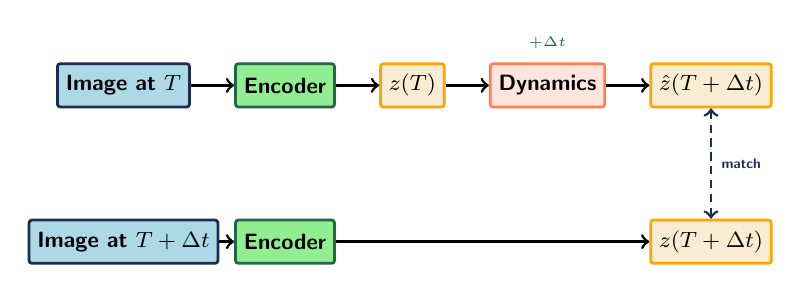
\begin{tikzpicture}[
    font=\sffamily\bfseries\footnotesize,
    box/.style={draw, line width=1pt, rectangle, rounded corners=1pt,
                minimum height=0.55cm, align=center, inner sep=3pt},
    node distance=0.55cm and 0.55cm,
  ]
    % Context path (top)
    \node[box, draw=darkblue, fill=lightblue] (imgT) {Image at $T$};
    \node[box, draw=darkgreen, fill=lightgreen, right=of imgT] (encT) {Encoder};
    \node[box, draw=orange, fill=gold!20, right=of encT] (zT) {$z(T)$};
    \node[box, draw=coral, fill=coral!20, right=of zT] (dyn) {Dynamics};
    \node[box, draw=orange, fill=gold!20, right=of dyn] (zpred) {$\hat{z}(T+\Delta t)$};

    \draw[->, line width=1pt] (imgT) -- (encT);
    \draw[->, line width=1pt] (encT) -- (zT);
    \draw[->, line width=1pt] (zT) -- (dyn);
    \draw[->, line width=1pt] (dyn) -- (zpred);
    \node[font=\sffamily\tiny\bfseries, text=darkgreen, above=0.05cm of dyn]
      {$+\Delta t$};

    % Target path (bottom): future image is encoded
    \node[box, draw=darkblue, fill=lightblue, below=1.4cm of imgT] (imgTd) {Image at $T+\Delta t$};
    \node[box, draw=darkgreen, fill=lightgreen] (encTd) at (encT |- imgTd) {Encoder};
    \node[box, draw=orange, fill=gold!20] (zTd) at (zpred |- imgTd) {$z(T+\Delta t)$};

    \draw[->, line width=1pt] (imgTd) -- (encTd);
    \draw[->, line width=1pt] (encTd) -- (zTd);

    % Match predicted vs encoded target
    \draw[<->, line width=1pt, densely dashed, darkblue]
      (zpred) -- node[right, font=\sffamily\tiny\bfseries, text=darkblue] {match} (zTd);
  \end{tikzpicture}%
  }
  \end{center}

  \smallskip

  \textbf{Two key components:}
  \begin{itemize}
    \item \textbf{Encoder:} Learns shared representation across CT, MRI, angiogram
    \item \textbf{Dynamics:} Predicts how latent state evolves over time
  \end{itemize}

\end{frame}

% ====================
% SLIDE 4: ENCODER & LATENT SPACE
% ====================
\begin{frame}{Encoder \& Factorized Latent Space}

  \textbf{Self-Supervised Learning (DINO, SimCLR)}
  \begin{itemize}
    \item Learns semantic features
    \item Robust across CT/MRI modality differences
    \item \textbf{Don't need labels!!!} 
  \end{itemize}

  \smallskip

  \textbf{Factorized Latent Space}: 
  Split up information into modality indepedent and specific, only use the independent for dynamics.
  \begin{center}
  \resizebox{!}{0.22\textheight}{%
  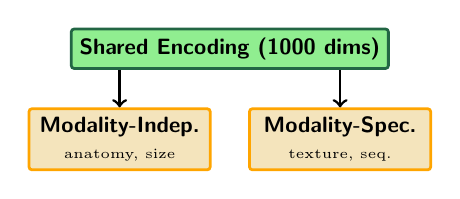
\begin{tikzpicture}[
    font=\sffamily\bfseries\footnotesize,
    box/.style={draw, line width=1pt, rectangle, rounded corners=1pt,
                align=center, inner sep=3pt},
  ]
    \node[box, draw=darkgreen, fill=lightgreen, minimum width=4.0cm, minimum height=0.5cm]
      (shared) at (0,1.15) {Shared Encoding (1000 dims)};

    \node[box, draw=orange, fill=gold!30, minimum width=2.3cm, minimum height=0.75cm]
      (indep) at (-1.4,0) {Modality-Indep.\\{\normalfont\tiny anatomy, size}};

    \node[box, draw=orange, fill=gold!30, minimum width=2.3cm, minimum height=0.75cm]
      (spec) at (1.4,0) {Modality-Spec.\\{\normalfont\tiny texture, seq.}};

    \draw[->, line width=1pt] (shared.south -| indep) -- (indep.north);
    \draw[->, line width=1pt] (shared.south -| spec) -- (spec.north);
  \end{tikzpicture}%
  }
  \end{center}

  \smallskip

  \textbf{Why factorize?}
  \begin{itemize}
    \item Predict in independent space $\Rightarrow$ can output any modality
  \end{itemize}

\end{frame}

\end{document}
